% \subsection{Peridynamics}

PD is a non-local theory to describe the physics of materials. Several assumptions made by the classical continuum mechanics theory are weakened or omitted. In continuum mechanics the medium has to be continuous, the internal forces are contact forces and interact in zero distance to each other. The deformation has to be two times differentiable \cite{BobaruF2017}. These assumptions have no physical motivation. In \cite{SillingSA2009} the comparison of the continuum mechanics and the ordinary state-based PD for the linear momentum balance is shown. The main difference from a mathematical point of view is that the PD theory is an integral formulation whereas the continuum mechanical theory is a partial differential equation. Therefore, if the material is discontinuous the continuum mechanics must fail. If the integral domain is zero PD and CM will be equal, see \autoref{eq:PeridynamicLimits}. %The angular momentum balance and the energy balance is given in \cite{SillingSA2009}.

Multiple PD formulations exist. The simplest, the bond based (BB) formulation, was presented in 2000 \cite{SillingSA2000}. Therein, materials are limited to a Poisson ratio of $\frac14$ for 3D and 2D plane strain problems as well es $\frac13$ for 2D plane stress problems \cite{HuangD2015}. To overcome these restrictions, enhancements of the method have been developed. The so called ordinary (OSB) and non-ordinary state-based (NOSB) formulation of PD are the result.

% \subsubsection{Ordinary state-based peridynamics}
\subsection{Ordinary state-based peridynamics}

In the original BB formulations, bond forces only depend on a single pair
of material points. The state-�based formulation considers bond forces dependent of deformations of all neighboring material points. The state-based PD is able to describe materials loosen the requirements on the Poisson ratio. It must be noted that, within the state-based peridynamic framework, there is no notion of connectivity such as a spring like force between two neighboring material points.  There simply is a potential between them. The equation of motion of the OSB-PD is represented as

\begin{align}
\label{eq:PeridynamicLimits}
\rho\left(\mathbf{x}\right)\mathbf{\ddot u}\left(\mathbf{x},t\right)&=\int_{\mathcal{H}}\left(\underline{\mathbf{T}}[\mathbf{x},t]\langle\mathbf{x}^{'}-\mathbf{x}\rangle-\underline{\mathbf{T}}[\mathbf{x}^{'},t]\langle\mathbf{x}-\mathbf{x}^{'}\rangle\right)dV+\mathbf{b}\left(\mathbf{x},t\right)
\end{align}

where $\mathcal{H}$ is a spherical neighborhood of radius or horizon $\delta$ centred at $\mathbf{x}$ and where $\underline{\mathbf{T}}$ is the force vector state field. All points $x'$ within the horizon of $x$ are called family of $x$. It maps the force of the bond $\langle\mathbf{x}^{'}-\mathbf{x}\rangle$ to force densities per volume \cite{SillingSA2007}. The variables $\mathbf{b}$, $\rho$, $\mathbf{u}$ and $\mathbf{\ddot u}$ are the external forces, the mass density, the displacement and the acceleration.

% \begin{figure}[htbp]
% \centering
% %% Creator: Inkscape 0.48.3.1, www.inkscape.org
%% PDF/EPS/PS + LaTeX output extension by Johan Engelen, 2010
%% Accompanies image file 'States.pdf' (pdf, eps, ps)
%%
%% To include the image in your LaTeX document, write
%%   \input{<filename>.pdf_tex}
%%  instead of
%%   \includegraphics{<filename>.pdf}
%% To scale the image, write
%%   \def\svgwidth{<desired width>}
%%   \input{<filename>.pdf_tex}
%%  instead of
%%   \includegraphics[width=<desired width>]{<filename>.pdf}
%%
%% Images with a different path to the parent latex file can
%% be accessed with the `import' package (which may need to be
%% installed) using
%%   \usepackage{import}
%% in the preamble, and then including the image with
%%   \import{<path to file>}{<filename>.pdf_tex}
%% Alternatively, one can specify
%%   \graphicspath{{<path to file>/}}
%% 
%% For more information, please see info/svg-inkscape on CTAN:
%%   http://tug.ctan.org/tex-archive/info/svg-inkscape
%%
\begingroup%
  \makeatletter%
  \providecommand\color[2][]{%
    \errmessage{(Inkscape) Color is used for the text in Inkscape, but the package 'color.sty' is not loaded}%
    \renewcommand\color[2][]{}%
  }%
  \providecommand\transparent[1]{%
    \errmessage{(Inkscape) Transparency is used (non-zero) for the text in Inkscape, but the package 'transparent.sty' is not loaded}%
    \renewcommand\transparent[1]{}%
  }%
  \providecommand\rotatebox[2]{#2}%
  \ifx\svgwidth\undefined%
    \setlength{\unitlength}{299.53755676bp}%
    \ifx\svgscale\undefined%
      \relax%
    \else%
      \setlength{\unitlength}{\unitlength * \real{\svgscale}}%
    \fi%
  \else%
    \setlength{\unitlength}{\svgwidth}%
  \fi%
  \global\let\svgwidth\undefined%
  \global\let\svgscale\undefined%
  \makeatother%
  \begin{picture}(1,0.45656065)%
    \put(0,0.02){\includegraphics[width=\unitlength]{./Figures/States.pdf}}%
    \put(0.43,0.46){\color[rgb]{0,0,0}\makebox(0,0)[lb]{\smash{$\mathbf{y}(.,t)$}}}%
    \put(0.95,0.3){\color[rgb]{0,0,0}\makebox(0,0)[lb]{\smash{$\underline{\mathbf{Y}}[\mathbf{x},t]\langle \mathbf{x}'-\mathbf{x}\rangle$}}}%
    \put(0.6,0.3){\color[rgb]{0,0,0}\makebox(0,0)[lb]{\smash{$\mathbf{y}(\mathbf{x},t)$}}}%
    \put(0.235,0.23){\color[rgb]{0,0,0}\makebox(0,0)[lb]{\smash{$\mathbf{x}$ }}}%
    \put(0.42,0.23){\color[rgb]{0,0,0}\makebox(0,0)[lb]{\smash{$\mathbf{x}'$ }}}%
    \put(1.03,0.24){\color[rgb]{0,0,0}\makebox(0,0)[lb]{\smash{$\mathbf{y}(\mathbf{x}',t)$ }}}%
  \end{picture}%
\endgroup%

% % %% Creator: Inkscape 0.48.3.1, www.inkscape.org
%% PDF/EPS/PS + LaTeX output extension by Johan Engelen, 2010
%% Accompanies image file 'States.pdf' (pdf, eps, ps)
%%
%% To include the image in your LaTeX document, write
%%   \input{<filename>.pdf_tex}
%%  instead of
%%   \includegraphics{<filename>.pdf}
%% To scale the image, write
%%   \def\svgwidth{<desired width>}
%%   \input{<filename>.pdf_tex}
%%  instead of
%%   \includegraphics[width=<desired width>]{<filename>.pdf}
%%
%% Images with a different path to the parent latex file can
%% be accessed with the `import' package (which may need to be
%% installed) using
%%   \usepackage{import}
%% in the preamble, and then including the image with
%%   \import{<path to file>}{<filename>.pdf_tex}
%% Alternatively, one can specify
%%   \graphicspath{{<path to file>/}}
%% 
%% For more information, please see info/svg-inkscape on CTAN:
%%   http://tug.ctan.org/tex-archive/info/svg-inkscape
%%
\begingroup%
  \makeatletter%
  \providecommand\color[2][]{%
    \errmessage{(Inkscape) Color is used for the text in Inkscape, but the package 'color.sty' is not loaded}%
    \renewcommand\color[2][]{}%
  }%
  \providecommand\transparent[1]{%
    \errmessage{(Inkscape) Transparency is used (non-zero) for the text in Inkscape, but the package 'transparent.sty' is not loaded}%
    \renewcommand\transparent[1]{}%
  }%
  \providecommand\rotatebox[2]{#2}%
  \ifx\svgwidth\undefined%
    \setlength{\unitlength}{299.53755676bp}%
    \ifx\svgscale\undefined%
      \relax%
    \else%
      \setlength{\unitlength}{\unitlength * \real{\svgscale}}%
    \fi%
  \else%
    \setlength{\unitlength}{\svgwidth}%
  \fi%
  \global\let\svgwidth\undefined%
  \global\let\svgscale\undefined%
  \makeatother%
  \begin{picture}(1,0.45656065)%
    \put(0,0.02){\includegraphics[width=\unitlength]{./Figures/States.pdf}}%
    \put(0.43,0.46){\color[rgb]{0,0,0}\makebox(0,0)[lb]{\smash{$\mathbf{y}(.,t)$}}}%
    \put(0.95,0.3){\color[rgb]{0,0,0}\makebox(0,0)[lb]{\smash{$\underline{\mathbf{Y}}[\mathbf{x},t]\langle \mathbf{x}'-\mathbf{x}\rangle$}}}%
    \put(0.6,0.3){\color[rgb]{0,0,0}\makebox(0,0)[lb]{\smash{$\mathbf{y}(\mathbf{x},t)$}}}%
    \put(0.235,0.23){\color[rgb]{0,0,0}\makebox(0,0)[lb]{\smash{$\mathbf{x}$ }}}%
    \put(0.42,0.23){\color[rgb]{0,0,0}\makebox(0,0)[lb]{\smash{$\mathbf{x}'$ }}}%
    \put(1.03,0.24){\color[rgb]{0,0,0}\makebox(0,0)[lb]{\smash{$\mathbf{y}(\mathbf{x}',t)$ }}}%
  \end{picture}%
\endgroup%

% % %% Creator: Inkscape 0.48.3.1, www.inkscape.org
%% PDF/EPS/PS + LaTeX output extension by Johan Engelen, 2010
%% Accompanies image file 'States.pdf' (pdf, eps, ps)
%%
%% To include the image in your LaTeX document, write
%%   \input{<filename>.pdf_tex}
%%  instead of
%%   \includegraphics{<filename>.pdf}
%% To scale the image, write
%%   \def\svgwidth{<desired width>}
%%   \input{<filename>.pdf_tex}
%%  instead of
%%   \includegraphics[width=<desired width>]{<filename>.pdf}
%%
%% Images with a different path to the parent latex file can
%% be accessed with the `import' package (which may need to be
%% installed) using
%%   \usepackage{import}
%% in the preamble, and then including the image with
%%   \import{<path to file>}{<filename>.pdf_tex}
%% Alternatively, one can specify
%%   \graphicspath{{<path to file>/}}
%% 
%% For more information, please see info/svg-inkscape on CTAN:
%%   http://tug.ctan.org/tex-archive/info/svg-inkscape
%%
\begingroup%
  \makeatletter%
  \providecommand\color[2][]{%
    \errmessage{(Inkscape) Color is used for the text in Inkscape, but the package 'color.sty' is not loaded}%
    \renewcommand\color[2][]{}%
  }%
  \providecommand\transparent[1]{%
    \errmessage{(Inkscape) Transparency is used (non-zero) for the text in Inkscape, but the package 'transparent.sty' is not loaded}%
    \renewcommand\transparent[1]{}%
  }%
  \providecommand\rotatebox[2]{#2}%
  \ifx\svgwidth\undefined%
    \setlength{\unitlength}{299.53755676bp}%
    \ifx\svgscale\undefined%
      \relax%
    \else%
      \setlength{\unitlength}{\unitlength * \real{\svgscale}}%
    \fi%
  \else%
    \setlength{\unitlength}{\svgwidth}%
  \fi%
  \global\let\svgwidth\undefined%
  \global\let\svgscale\undefined%
  \makeatother%
  \begin{picture}(1,0.45656065)%
    \put(0,0.02){\includegraphics[width=\unitlength]{./Figures/States.pdf}}%
    \put(0.43,0.46){\color[rgb]{0,0,0}\makebox(0,0)[lb]{\smash{$\mathbf{y}(.,t)$}}}%
    \put(0.95,0.3){\color[rgb]{0,0,0}\makebox(0,0)[lb]{\smash{$\underline{\mathbf{Y}}[\mathbf{x},t]\langle \mathbf{x}'-\mathbf{x}\rangle$}}}%
    \put(0.6,0.3){\color[rgb]{0,0,0}\makebox(0,0)[lb]{\smash{$\mathbf{y}(\mathbf{x},t)$}}}%
    \put(0.235,0.23){\color[rgb]{0,0,0}\makebox(0,0)[lb]{\smash{$\mathbf{x}$ }}}%
    \put(0.42,0.23){\color[rgb]{0,0,0}\makebox(0,0)[lb]{\smash{$\mathbf{x}'$ }}}%
    \put(1.03,0.24){\color[rgb]{0,0,0}\makebox(0,0)[lb]{\smash{$\mathbf{y}(\mathbf{x}',t)$ }}}%
  \end{picture}%
\endgroup%

% \caption{Family: initial \& deformed configuration with deformation state $\underline{\mathbf{Y}}$ \cite{SillingSA2009}}
% \label{fig:states}
% \end{figure}
% 
\begin{figure}[htbp]
  \centering
  \begin{tikzpicture}
    % External figure
    %\node[anchor=south west,inner sep=0] (image) at (0,0) {\includegraphics[scale=1.0]{../../../../../Publications/Doc/PeriDoc_Common/Figures/States}};
    \node[anchor=south west,inner sep=0] (image) at (0,0) {\includegraphics[scale=1.0]{States.pdf}};
    % Scope
    \begin{scope}[
      x={(image.south east)},
      y={(image.north west)},
    ]
      % Some label
      \node (xlabel)    at (0.19,0.35) {$\mathbf{x}$};
      \node (xslabel)   at (0.36,0.09) {$\mathbf{x}'$};
      \node (ylabel)    at (0.66,0.66) {$\mathbf{y}\left(\mathbf{x},t\right)$};
      \node (yslabel)   at (0.94,0.23) {$\mathbf{y}\left(\mathbf{x}',t\right)$};
      \node (yalllabel) at (0.48,0.94) {$\mathbf{y}\left(.,t\right)$};
      \node (Ylabel)    at (1.02,0.71) {$\mathbf{Y}\left[\mathbf{x},t\right]\langle\mathbf{x}'-\mathbf{x}\rangle$};
      % Help grid and labels
      %\draw[help lines,xstep=.1,ystep=.1] (0,0) grid (1,1);
      %\foreach \x in {0,1,...,9} {\node [anchor=north] at (\x/10,0) {0.\x};}
      %\foreach \y in {0,1,...,9} {\node [anchor=east]  at (0,\y/10) {0.\y};}
    \end{scope}
  \end{tikzpicture}
  \caption{Family: initial \& deformed configuration with deformation state $\underline{\mathbf{Y}}$ \cite{SillingSA2009}}
  \label{fig:states}
\end{figure}

$\underline{\mathbf{T}}$ has to ensure the consistency with basic physical principles as the balance of linear momentum. This can be shown for any $\underline{\mathbf{T}}$. To describe a material, constitutive models are needed. These models map specific deformation vector state fields $\underline{\mathbf{Y}}$ in the force vector state $\underline{\mathbf{T}}$.

\begin{equation}
\label{eq:PeridynamicLimits2}
\lim\limits_{\mathcal{H} \to 0} \int_{\mathcal{H}}\left(\underline{\mathbf{T}}[\mathbf{x},t]\langle\mathbf{x}^{'}-\mathbf{x}\rangle-\underline{\mathbf{T}}[\mathbf{x}^{'},t]\langle\mathbf{x}-\mathbf{x}^{'}\rangle\right)dV=\text{div}(\boldsymbol{\sigma})
\end{equation}

% \subsubsection{Material model}
\subsection{Material model}

It is assumed that the elastic strain energy in a PD solid is equal to the energy of the CM model. In that case, it is supposed that there is a PD strain energy density function $W(�)\,:\, V \rightarrow \Re$ such, that for some choice of the deformation gradient

\begin{equation}
 \underline{\mathbf{Y}}(\boldsymbol{\xi}) = \mathbf{F}\boldsymbol{\xi}=\mathbf{F}\langle\mathbf{x}'-\mathbf{x}\rangle\quad \forall\boldsymbol{\xi}\in \mathcal{H}.
\end{equation}

Then the PD constitutive model corresponds to the classical constitutive model at $\mathbf{F}$ \cite{SillingSA2007,AguiarAR2014}. With the extension scalar state $\underline{e}$

\begin{equation}
 \underline{e}=\underline{y}-\underline{x},\qquad \underline{y}=|\underline{\mathbf{Y}}|,\qquad\underline{x}=|\underline{\mathbf{X}}|
\end{equation}

the pairwise force density for an isotropic elastic PD solid

\begin{equation}
\label{eq:matModel}
\underline{t}=\frac{3 K \theta}{V_w}\underline{\omega x}+\frac{15G}{V_w}\underline{\omega e}^d
\end{equation}

can be determined utilizing the bulk modulus $K$  and the shear modulus $G$. The variables $\theta$ and the deviatoric part of the extension scalar state $\underline{e}^d$ are given as

\begin{equation}
\theta=\frac{3}{V_w}\int_\mathcal{H}(\underline{\omega}\underline{x})\cdot\underline{e}dV\quad\text{and}\quad\underline{e}^d=\underline{e}-\frac{\theta\underline{x}}{3}\quad\mbox{.}
\end{equation}

The value $V_w$ is the weighted volume and $\underline{\omega}$ is the influence function which can be used to weight the bond stiffness related to the position in $\mathcal{H}$. It is a part of the constitutive response. The complete derivation is given in \cite{SillingSA2007}. The model is similar to the classical one

\begin{equation}
 \boldsymbol{\sigma}=K\mathbf{I}\text{tr}(\boldsymbol{\epsilon})+2G\boldsymbol{\epsilon}^d,
\end{equation}

where $\boldsymbol{\sigma}$ is the mechanical stress, $\text{tr}(\boldsymbol{\epsilon})$ is the trace of the mechanical strain and $\boldsymbol{\epsilon}^d$ is the deviatoric part of the mechanical strain.

% \subsubsection{Damage model}
\subsection{Damage model}

One method of introducing failure into PD is through the irreversible breaking of ``bonds'' by setting the potential between them to zero. Failure is introduced by allowing the removal of this potential when certain physical variables reach a critical level \cite{FosterJT2009}.

\begin{equation}
\label{eq:DetermineMicroDamagePotential}
w_c=\frac{4G_0}{\pi\delta^4}
\end{equation}

The critical micro potential can be determined using the energy release rate $G_0$ in \autoref{eq:DetermineMicroDamagePotential}. \cite{FosterJT2009,FosterJT2011} describe an energy-based failure criterion which is valid for state-based analysis by comparison of the critical energy density to the energy density of each state between material points. If the bonds micro potential is greater than this value the bond is deleted. With the history-dependent scalar valued function $\chi(\boldsymbol{\xi},t)$

\begin{equation}
\label{eq:checkDamage}
\chi(\boldsymbol{\underline{e}}\langle\boldsymbol{\xi}\rangle,t)  = \begin{cases} 1 \qquad \text{if}\ w(\underline{e}\langle\boldsymbol{\xi}\rangle) < w_c\ \text{for all}\ 0 < t' < t\\
0 \qquad \text{otherwise}\end{cases}	\quad\mbox{,}
\end{equation}

the damage model can be included in \autoref{eq:matModel}.

\begin{equation}
\label{eq:matModel2}
\underline{t}=\chi(\boldsymbol{\underline{e}}\langle\boldsymbol{\xi},t)\left(\frac{3 K \theta}{V_w}\underline{\omega} \underline{x}+\frac{15G}{V_w}\underline{\omega} \underline{e}^d\right)
\end{equation}

Each ``bond'' has a simple damage law as shown in \autoref{fig:Damage_Models_CriticalStretch}, whereas the resulting integral material response is illustrated in \autoref{fig:Damage_Models_Integral}. It can be seen that the integral behavior corresponds to a standard analytical traction-separation law \cite{BobaruF2017}. The dissipated energy in the material is simply the integral of the bond breakage energies over all the broken bonds in the family \cite{SillingSA2010b}.

\setlength{\figheight}{4.0cm}

\begin{figure}[ht]
  \begin{subfigure}{0.49\linewidth}
    \centering
    \begin{minipage}[b][\figheight]{\linewidth}
        % Math
  \pgfkeys{/pgf/fpu}
  \pgfmathsetmacro{\bondconstant}{18927.8}
  \pgfmathsetmacro{\criticalstretch}{0.2}
  \pgfkeys{/pgf/fpu=false}
  % Shapes
%   \tikzset{%
%     myarrowdecoration1/.style={postaction={decorate,decoration={
%       markings,
%       mark=between positions .4 and .6 step .1pt with {\draw [thin] circle (.1pt);},
%       mark=at position .6 with {\arrow[thin,xshift=1pt]{latex}},
%       raise=-0.7ex,
%     }}},
%     myarrowdecoration2/.style={postaction={decorate,decoration={
%       markings,
%       mark=between positions .4 and .6 step .1pt with {\draw [thin] circle (.1pt);},
%       mark=at position .4 with {\arrow[thin,xshift=1pt]{latex reversed}},
%       raise=0.7ex,
%     }}},
%   }
  % Axis
\begin{tikzpicture}
  %
  \tikzset{%
    myarrowdecoration/.style={postaction={decorate,decoration={
      markings,
      mark=between positions .2 and .8 step .1pt with {\draw [thin,-latex] circle (.1pt);},
      mark=at position .8 with {\arrow[thin,xshift=1pt]{latex}},
      mark=at position .2 with {\arrow[thin,xshift=1pt]{latex reversed}},
      raise=0.7ex,
    }}},
  }
  %
  \begin{axis}[
%     scale only axis,
    axis lines=middle,
    %ticks=none,
    domain=-1.4*\criticalstretch:1.4*\criticalstretch,
    %restrict y to domain=-\ultimatestrength:\ultimatestrength,
    xmin=0.0*\criticalstretch,
    xmax= 1.5*\criticalstretch,
    ymin=0.0*(\bondconstant*\criticalstretch),
    ymax= 1.5*(\bondconstant*\criticalstretch),
    width=0.65\linewidth,
    %height=0.99\textwidth,
    ylabel={Bond traction},
    xlabel={Bond stretch},
    xtick={\criticalstretch},
    xticklabels={Bond damage},
    ytick=\empty,
    every axis x label/.style={
      at={(ticklabel* cs:1.005)},
      anchor=west,
    },
    every axis y label/.style={
      at={(ticklabel* cs:1.005)},
      anchor=south,
    },
  ]
    % Plots
    \addplot[dashed] {\bondconstant*x} node[pos=0.95] (pinc) {};
    \addplot[very thick,domain=-1.4*\criticalstretch:\criticalstretch] {\bondconstant*x} node[pos=0.2] (c1pos) {} node[pos=0.3] (c2pos) {} node[pos=1.0] (failpos) {};
    
    \draw[very thick] (failpos.center) -- (\criticalstretch,0);
    \draw[myarrowdecoration,very thick] (0.6*\criticalstretch,0) -- (\criticalstretch,0);
    \draw[myarrowdecoration,very thick] (\criticalstretch,0) -- (1.4*\criticalstretch,0);
    % Label
    \coordinate (c12pos) at (c2pos|-c1pos);
    \draw[thin] (c1pos) -- (c12pos);
    \draw[thin] (c2pos) -- (c12pos) node[midway,right]{$c$};
    % Coordinates
%     \coordinate (origin) at (0,0);
%     \coordinate (yieldt) at ( \yieldstraint, \yieldstresst);
%     \coordinate (yieldc) at (-\yieldstrainc,-\yieldstressc);
%     % Lines
%     \draw[thick,myarrowdecoration1,myarrowdecoration2] (origin) -- node[pos=0.8, pin=-60:{\pinlabel}](ELabel){} (yieldt);
%     \draw[thick,myarrowdecoration1,myarrowdecoration2] (origin) -- (yieldc);
    % Label
    %\iftoggle{tclabel}{%
%       \node[anchor=north east,xshift=-0.6cm] (tensionlabel) at (rel axis cs:1,1) {\footnotesize tension};
      %\node[anchor=south west,xshift= 0.6cm] (compressionlabel) at (rel axis cs:0,0) {\footnotesize compression};
    %}{}
  \end{axis}
\end{tikzpicture}
    \end{minipage}
    \caption{Local behavior of one bond}
    \label{fig:Damage_Models_CriticalStretch}
  \end{subfigure}%
  \hfill
  \begin{subfigure}{0.49\linewidth}
    \centering
    \begin{minipage}[b][\figheight]{\linewidth}
        % Math
  \pgfkeys{/pgf/fpu}
  \pgfmathsetmacro{\bondconstant}{18927.8}
  \pgfmathsetmacro{\criticalstretch}{0.2}
  \pgfkeys{/pgf/fpu=false}
  % Shapes
%   \tikzset{%
%     myarrowdecoration1/.style={postaction={decorate,decoration={
%       markings,
%       mark=between positions .4 and .6 step .1pt with {\draw [thin] circle (.1pt);},
%       mark=at position .6 with {\arrow[thin,xshift=1pt]{latex}},
%       raise=-0.7ex,
%     }}},
%     myarrowdecoration2/.style={postaction={decorate,decoration={
%       markings,
%       mark=between positions .4 and .6 step .1pt with {\draw [thin] circle (.1pt);},
%       mark=at position .4 with {\arrow[thin,xshift=1pt]{latex reversed}},
%       raise=0.7ex,
%     }}},
%   }
  % Axis
\begin{tikzpicture}
  %
  \tikzset{%
	myarrowdecoration/.style={postaction={decorate,decoration={
	  markings,
	  mark=between positions .2 and .8 step .1pt with {\draw [thin,-latex] circle (.1pt);},
	  mark=at position .8 with {\arrow[thin,xshift=1pt]{latex}},
	  mark=at position .2 with {\arrow[thin,xshift=1pt]{latex reversed}},
	  raise=0.7ex,
	}}},
  }
  %
  \begin{axis}[
%     scale only axis,
	axis lines=middle,
	%ticks=none,
	domain=0:1.4*\criticalstretch,
	%restrict y to domain=-\ultimatestrength:\ultimatestrength,
	xmin=0.0*\criticalstretch,
	xmax= 1.5*\criticalstretch,
	ymin= 0.0*(\bondconstant*\criticalstretch),
	ymax= 1.5*(\bondconstant*\criticalstretch),
	width=0.65\linewidth,
	%height=0.99\textwidth,
        xlabel={Separation},
	ylabel={Traction},
	xtick={\criticalstretch},
	xticklabels={Damage initiation},
	ytick=\empty,
	every axis x label/.style={
	  at={(ticklabel* cs:1.005)},
	  anchor=west,
	},
	every axis y label/.style={
	  at={(ticklabel* cs:1.005)},
	  anchor=south,
	},
  ]
	% Plots
	%\addplot[dashed] {\bondconstant*x} node[pos=0.95] (pinc) {};
	\addplot[very thick,domain=0:\criticalstretch] {\bondconstant*x} node[pos=0.2] (c1pos) {} node[pos=0.3] (c2pos) {} node[pos=1.0] (failpos) {};

	\draw[very thick] (failpos.center) -- (1.4*\criticalstretch,0);
	%\draw[myarrowdecoration,very thick] (0.6*\criticalstretch,0) -- (\criticalstretch,0);
	%\draw[myarrowdecoration,very thick] (\criticalstretch,0) -- (1.4*\criticalstretch,0);
	% Label
	%\coordinate (c12pos) at (c2pos|-c1pos);
	%\draw[thin] (c1pos) -- (c12pos);
	%\draw[thin] (c2pos) -- (c12pos) node[midway,right]{$c$};
	
	% Coordinates
%     \coordinate (origin) at (0,0);
%     \coordinate (yieldt) at ( \yieldstraint, \yieldstresst);
%     \coordinate (yieldc) at (-\yieldstrainc,-\yieldstressc);
%     % Lines
%     \draw[thick,myarrowdecoration1,myarrowdecoration2] (origin) -- node[pos=0.8, pin=-60:{\pinlabel}](ELabel){} (yieldt);
%     \draw[thick,myarrowdecoration1,myarrowdecoration2] (origin) -- (yieldc);
	% Label
	%\iftoggle{tclabel}{%
%	  \node[anchor=north east,xshift=-0.6cm] (tensionlabel) at (rel axis cs:1,1) {\footnotesize tension};
	  %\node[anchor=south west,xshift= 0.6cm] (compressionlabel) at (rel axis cs:0,0) {\footnotesize compression};
	%}{}
  \end{axis}
\end{tikzpicture} 
    \end{minipage}
    \caption{Integral response of the material \cite{BobaruF2017}}
    \label{fig:Damage_Models_Integral} 
  \end{subfigure}%
  \caption{Comparison of the bond and integral material damage response}
  \label{fig:Zugversuch}
\end{figure}

The damage law used in this publication is much simpler. It is assumed that for the one-dimensional cases considered, a critical bond elongation determined in CM can be used as input for the so-called critical stretch criterion, as done by \cite{GerstleW2005} for bond-based peridynamics. In that case \autoref{eq:checkDamage} is reformulated to

\begin{equation}
\label{eq:checkDamage2}
\chi(\boldsymbol{\underline{e}}\langle\boldsymbol{\xi}\rangle,t)  = \begin{cases} 1 \qquad \text{if}\ \frac{\mathbf{y}(\mathbf{x}',t)-\mathbf{y}(\mathbf{x},t)}{|\mathbf{x}'-\mathbf{x}|} < \epsilon_{crit}\ \text{for all}\ 0 < t' < t\\
0 \qquad \text{otherwise}\end{cases}
\end{equation}

% This method has been used, because in the actual framework only the critical stretch values as presented here has been implemented.
with $\epsilon_{c}$ as critical stretch value. \cite{BobaruF2017} point out that this method is derived from BB-PD and that the concept may not apply in state-based material models as used in the current study. However, no other failure model has been implemented in the current numerical framework yet.

% As done by \cite{GerstleW2005} for bond-based peridynamics, it is assumed that the micro elastic critical stretch is equal to the uniaxial tensile strain.
% 
% \begin{align}
%   s_0 &= \varepsilon_u
% \end{align}
% 
% This is usually not valid for state-based peridynamics. \cite{FosterJT2009,FosterJT2011} describe an energy-based failure criterion which is valid for state-based analysis by comparison of the critical energy density to the energy density of each state between material points. However, for isotropic material and uniaxial loading, the simple approach from \cite{GerstleW2005} gives reasonably good results.